\chapter{Clustering}
\label{chap-clustering}

Oftentimes a dataset can be partitioned into different categories. A
doctor may notice that their patients come in cohorts and different
cohorts respond to different treatments. A biologist may gain insight
by identifying that bats and whales, despite outward appearances,
have some underlying similarity, and both should be considered members
of the same category, i.e., ``mammal''. The problem of automatically
identifying meaningful groupings in datasets is called
clustering. Once these groupings are found, they can be leveraged
toward interpreting the data and making optimal decisions for each
group.
\index{clustering}

\section{Clustering formalisms}

%Imagine that you are a scientist studying the human genome.

%Sometimes data seems to come in different categories. How can we
%identify these categories, and thereby treat them specifically? We
%call these categories clusters.

%Mathematically, clustering is the problem of \textit{partitioning} a
%dataset $\{x_i\}_{i=1}^n$ such that each datapoint is assigned to one
%partition.

Mathematically, clustering looks a bit like classification: we wish to
find a mapping from datapoints, $x$, to categories, $y$. However,
rather than the categories being predefined labels, the categories in
clustering are automatically discovered \textit{partitions} of an
unlabeled dataset.\index{clustering!into partitions}

Because clustering does not learn from labeled examples, it is an
example of an \textit{unsupervised} learning algorithm. Instead of
mimicking the mapping implicit in supervised training pairs
$\{x^{(i)},y^{(i)}\}_{i=1}^n$, clustering assigns datapoints to
categories based on how the unlabeled data $\{x^{(i)}\}_{i=1}^n$ is
\textit{distributed} in data space.

%, which can be indexed by the integers, $\mathbb{Z}$. That is, in
%both classification and clustering, we learn $f: \mathbb{R}^N
%\rightarrow \mathbb{Z}$.

%The difference between clustering and classification is in the
%objective function. Classification is supervised -- we simply map
%datapoints to categories in a way that matches training examples
%$\{x^{(i)},y^{(i)}\}_{i=1}^n$. Clustering, on the other hand, is
%\textit{unsupervised}: we are only given unlabeled datapoints
%$\{x^{(i)}\}_{i=1}^n$, and we have to decide which datapoints belong
%to which categories based on how the data is \textit{distributed} in
%data space.

Intuitively, a ``cluster'' is a group of datapoints that are all
nearby to each other and far away from other clusters. Let's consider
the following scatter plot. How many clusters do you think there are?

\begin{figure}[h]
  \centering
  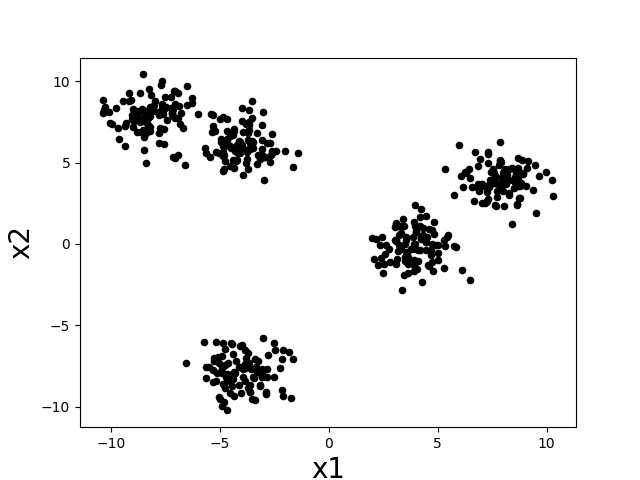
\includegraphics[width=0.40\textwidth]{figures/kmeans_fig1.png}
  \caption{A dataset we would like to cluster. How many clusters do you think there are?}
  \label{fig:kmeans_fig1}
\end{figure}

There seem to be about five clumps of datapoints and those clumps are
what we would like to call clusters. If we assign all datapoints in
each clump to a cluster corresponding to that clump, then we might
desire that nearby datapoints are assigned to the same cluster, while
far apart datapoints are assigned to different clusters.

In designing clustering algorithms, three critical things we need to decide are:
\begin{itemize}
  \item How do we measure \textit{distance} between datapoints? What counts as ``nearby'' and ``far apart''?
  \item How many clusters should we look for?
  \item How do we evaluate how good a clustering is?
\end{itemize}

We will see how to begin making these decisions as we work through a
concrete clustering algorithm in the next section.

\section{The k-means formulation}

% Describe with pictures; show good clustering, bad clustering, how do
% we measure? show cluster centers? center pulls in the data. what's
% the objective? here is a reasonable one. quantify dispersal with
% variance --> k-means objective.


% consider showing algorithm first?

One of the simplest and most commonly used clustering algorithms is
called k-means. The goal of the k-means\anchorednote{algorithm}{We
will be careful to distinguish between the k-means {\em algorithm}
and the k-means {\em objective}. As we will see, the k-means
algorithm can be understood to be just one optimization algorithm
which finds a local optimum of the k-means objective.} is to assign
datapoints to $k$ clusters in such a way that
the\anchorednote{variance}{Recall that \textit{variance} is a measure
  of how ``spread out'' data is, defined as the mean squared distance
  from the average value of the data.} within clusters is as small as
possible. Notice that this matches our intuitive idea that a cluster
should be a tightly packed set of datapoints.

Similar to the way we showed that supervised learning could be
formalized mathematically as the minimization of an objective function
(loss function + regularization), we will show how unsupervised
learning can also be formalized as minimizing an objective function.
Let us denote the cluster assignment for a datapoint $x^{(i)}$ as
$y^{(i)} \in \{1,2,\ldots,k\}$, i.e., $y^{(i)} = 1$ means we are
assigning datapoint $x^{(i)}$ to cluster number 1. Then the k-means
objective can be quantified with the following objective function
(which we also call the ``k-means loss''):
\begin{equation}
  \sum_{j=1}^k \sum_{i=1}^n \mathbb{1}(y^{(i)} = j) \left\Vert x^{(i)} - \mu^{(j)} \right\Vert^2 \label{eqn:kmeans_obj} \;,
\end{equation}
where $\mu^{(j)} = \frac{1}{N_j} \sum_{i=1}^n \mathbb{1}(y^{(i)} = j) x^{(i)}$
and $N_j = \sum_{i=1}^n \mathbb{1}(y^{(i)} = j)$, so that $\mu^{(j)}$ is the
mean of all datapoints in cluster $j$, and using $\mathbb{1}(\cdot)$
to denote the indicator function (which takes on value of 1 if its argument
is true and 0 otherwise). The inner sum (over data points) of the loss is
the variance of datapoints within cluster $j$. We sum up the variance
of all $k$ clusters to get our overall loss.\index{k-means!formulation}

\subsection{K-means algorithm}

\index{clustering!k-means algorithm}
The k-means algorithm minimizes this loss by alternating between two
steps: given some initial cluster assignments: 1) compute the mean of
all data in each cluster and assign this as the ``cluster mean'', and 2)
reassign each datapoint to the cluster with nearest cluster
mean. Fig.~\ref{fig:kmeans_iters} shows what happens when we repeat
these steps on the dataset from above.

\begin{figure}[h]
  \centering
  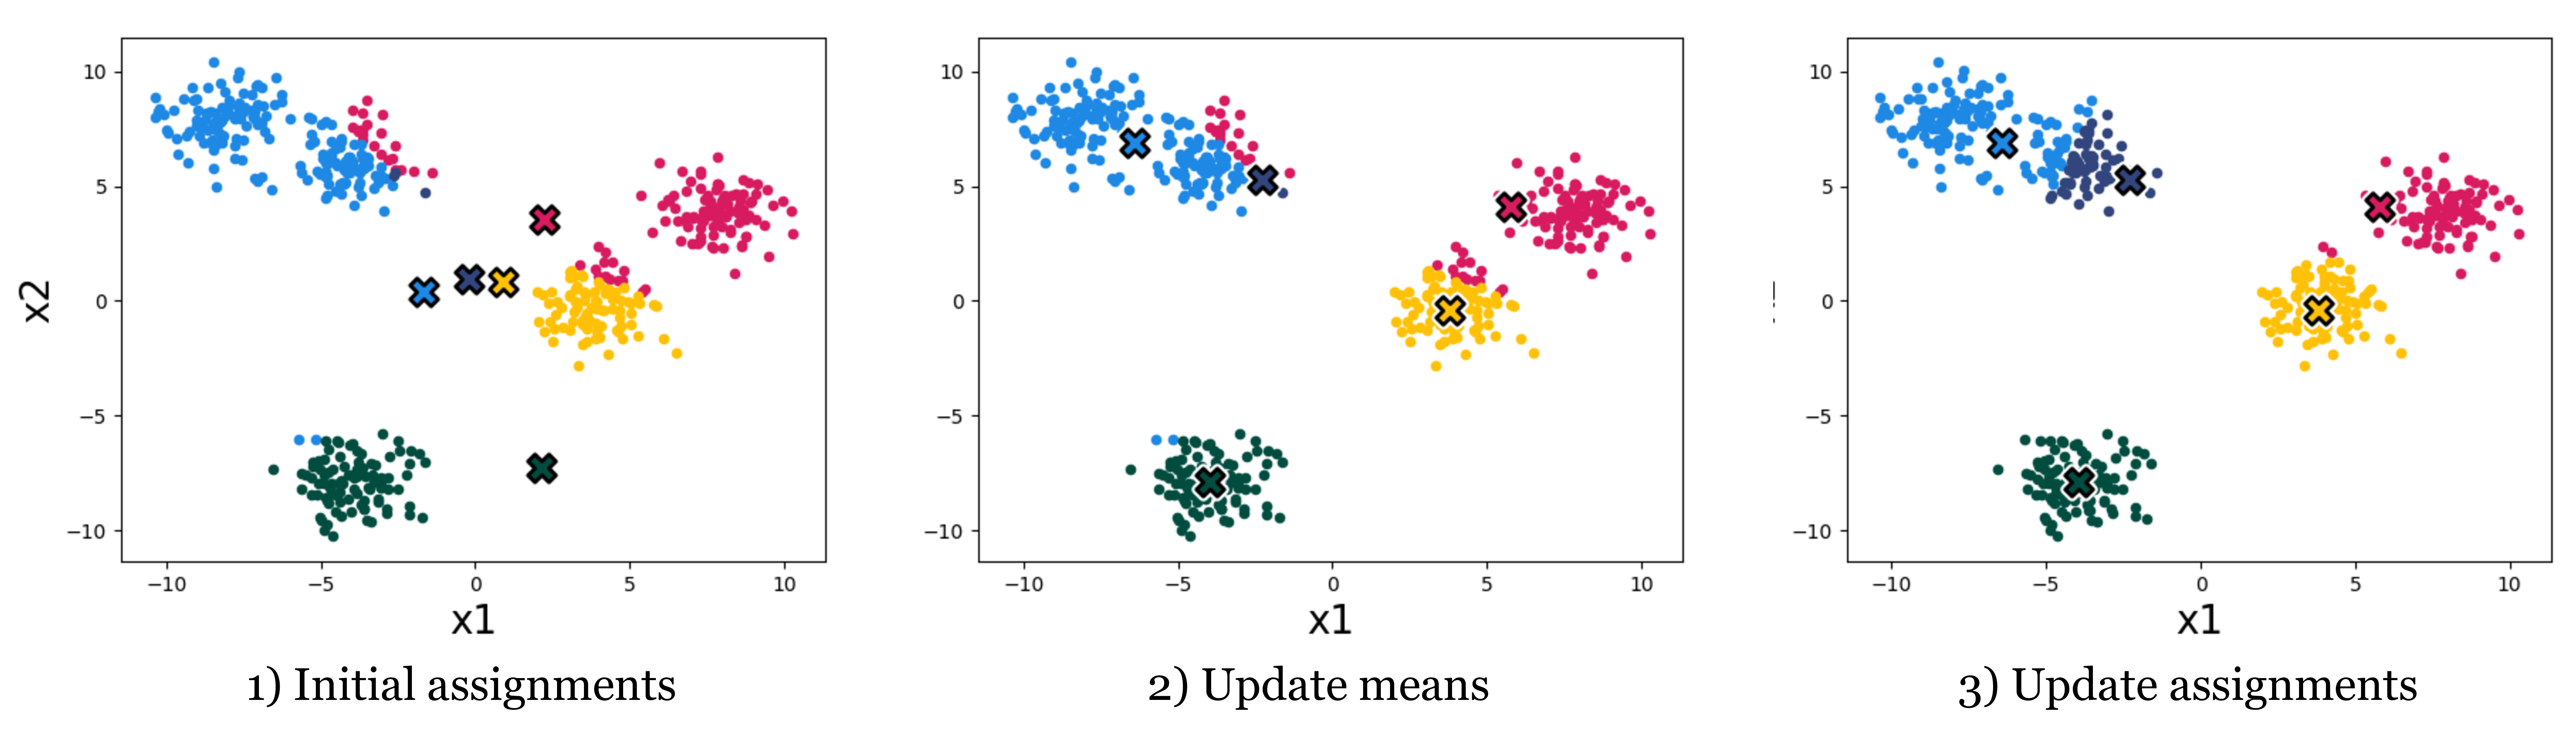
\includegraphics[width=1.0\textwidth]{figures/kmeans_iters.png}
  \caption{The first three steps of running the k-means algorithm on
    this data. Datapoints are colored according to the cluster to
    which they are assigned. Cluster means are the larger X's with
    black outlines.}
  \label{fig:kmeans_iters}
\end{figure}

Each time we reassign the data to the nearest cluster mean, the
k-means loss decreases (the datapoints end up closer to their assigned
cluster mean), or stays the same.  And each time we recompute the
cluster means the loss \textit{also} decreases (the means end up
closer to their assigned datapoints) or stays the same. Overall then,
the clustering gets better and better, according to our objective --
until it stops improving.

After four iterations of cluster assignment + update means in our example,
the k-means algorithm stops improving. We say it has converged,
and its final solution is shown in Fig.~\ref{fig:kmeans_converged}.
\begin{figure}[h]
  \centering
  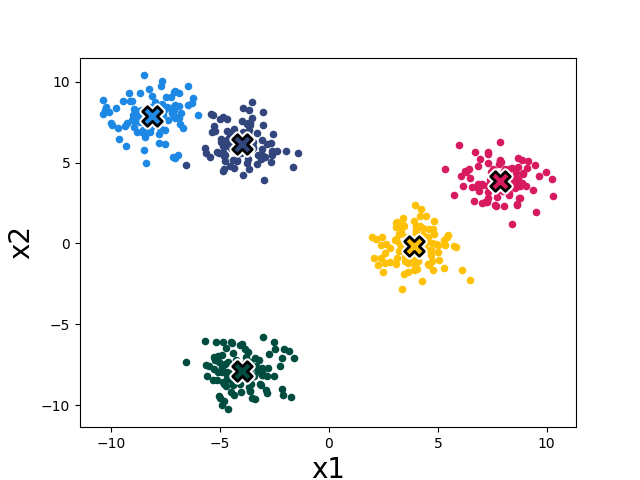
\includegraphics[width=0.4\textwidth]{figures/kmeans_fig2_converged.png}
  \caption{Converged result.}
  \label{fig:kmeans_converged}
\end{figure}

It seems to converge to something reasonable! Now let's write out the
algorithm in complete detail:
%It can be shown that under mild conditions, this process converges to
%a local minimum of the k-means loss!

%Given some initial assignment of the data to clusters, we first
%compute the mean of all datapoints in each cluster. Then we reassign
%each datapoint to the cluster with the nearest mean. This process
%repeats until convergence.

\begin{codebox}
  \Procname{$\proc{k-means}(k, \tau, \{x^{(i)}\}_{i=1}^n)$}
  \li $\mu, y \gets $ random initialization
  \li \For $t \gets 1$ \To $\tau$
  \li   \Do
  $y_{\texttt{old}} = y$
  \li        \For $i \gets 1$ \To $n$
  \li       \Do
  $y^{(i)} = \arg\min_j \left\Vert x^{(i)} - \mu^{(j)} \right\Vert^2$
  \End
  \li    \For $j \gets 1$ \To $k$
  \li       \Do
  $\mu^{(j)} = \frac{1}{N_j} \sum_{i=1}^n \mathbb{1}(y^{(i)} = j) x^{(i)}$
  \End
  \li      \If $\mathbb{1}(y = y_{\texttt{old}})$
  \li          \Then
  break \label{alg:termination}
  \End
  \End
  \li \Return $\mu, y$
\end{codebox}
\index{k-means!algorithm}
\question{Why do we have the ``break'' statement on
  line~\ref{alg:termination}? Could the clustering improve if we ran
  it for more iterations after this point? Has it converged?}

The for-loop over the $n$ datapoints assigns each datapoint to the
nearest cluster center. The for-loop over the k clusters updates the
cluster center to be the mean of all datapoints currently assigned to
that cluster. As suggested above, it can be shown that this algorithm
reduces the loss in Eq.~\ref{eqn:kmeans_obj} on each iteration, until
it converges to a local minimum of the loss.

% time complexity

It's like classification except it \textit{picked} what the classes
are rather than being given examples of what the classes are.

\subsection{Using gradient descent to minimize k-means objective}

%Study question: could you also minimize the objective with gradient descent?
\index{gradient descent!applied to k-means}
We can also use \anchorednote{gradient descent}{The k-means algorithm
  presented above is a form of \textit{block coordinate descent},
  rather than gradient descent. For certain problems, and in
  particular k-means, this method can converge faster than gradient
  descent.}  to optimize the k-means objective.  To show how to apply
gradient descent, we first rewrite the objective as a differentiable
function \textit{only of} $\mu$:
\begin{equation}
  L(\mu) = \sum_{i=1}^n \min_j \left\Vert x^{(i)} - \mu^{(j)} \right\Vert^2 \;\;.
\end{equation}
$L(\mu)$ is the value of the k-means loss given that we pick the
\textit{optimal} assignments of the datapoints to cluster means
(that's what the $\min_j$ does). Now we can use the
gradient\anchorednote{$\frac{\partial L(\mu)}{\partial \mu}$}{$L(\mu)$
  is a smooth function except with kinks where the nearest cluster
  changes; that means it's differentiable almost everywhere, which in
  practice is sufficient for us to apply gradient descent.} to find
the values for $\mu$ that achieve minimum loss when cluster
assignments are optimal.  Finally, we read off the optimal cluster
assignments, given the optimized $\mu$, just by assigning datapoints
to their nearest cluster mean:
\begin{equation}
  y^{(i)} = \arg\min_j \left\Vert x^{(i)} - \mu^{(j)} \right\Vert^2 \;\;.
\end{equation}
This procedure yields a local minimum of Eq.~\ref{eqn:kmeans_obj}, as
does the standard k-means algorithm we presented (though they might
arrive at different solutions). It might not be the global optimum
since the objective is not convex (due to $\min_j$, as the minimum of
multiple convex functions is not necessarily convex).

% mention sub-gradient
% figure out if this is ever done in practice
% say it is not typical

% previous algorithm is block coordinate descent

\subsection{Importance of initialization}
The standard k-means algorithm, as well as the variant that uses
gradient descent, both are only guaranteed to converge to a local
minimum, not necessarily the global minimum of the loss. Thus the
answer we get out depends on how we initialize the cluster
means. Figure~\ref{fig:kmeans_init} is an example of a different
initialization on our toy data, which results in a worse converged
clustering:\index{k-means!initialization}

\begin{figure}[h]
  \centering
  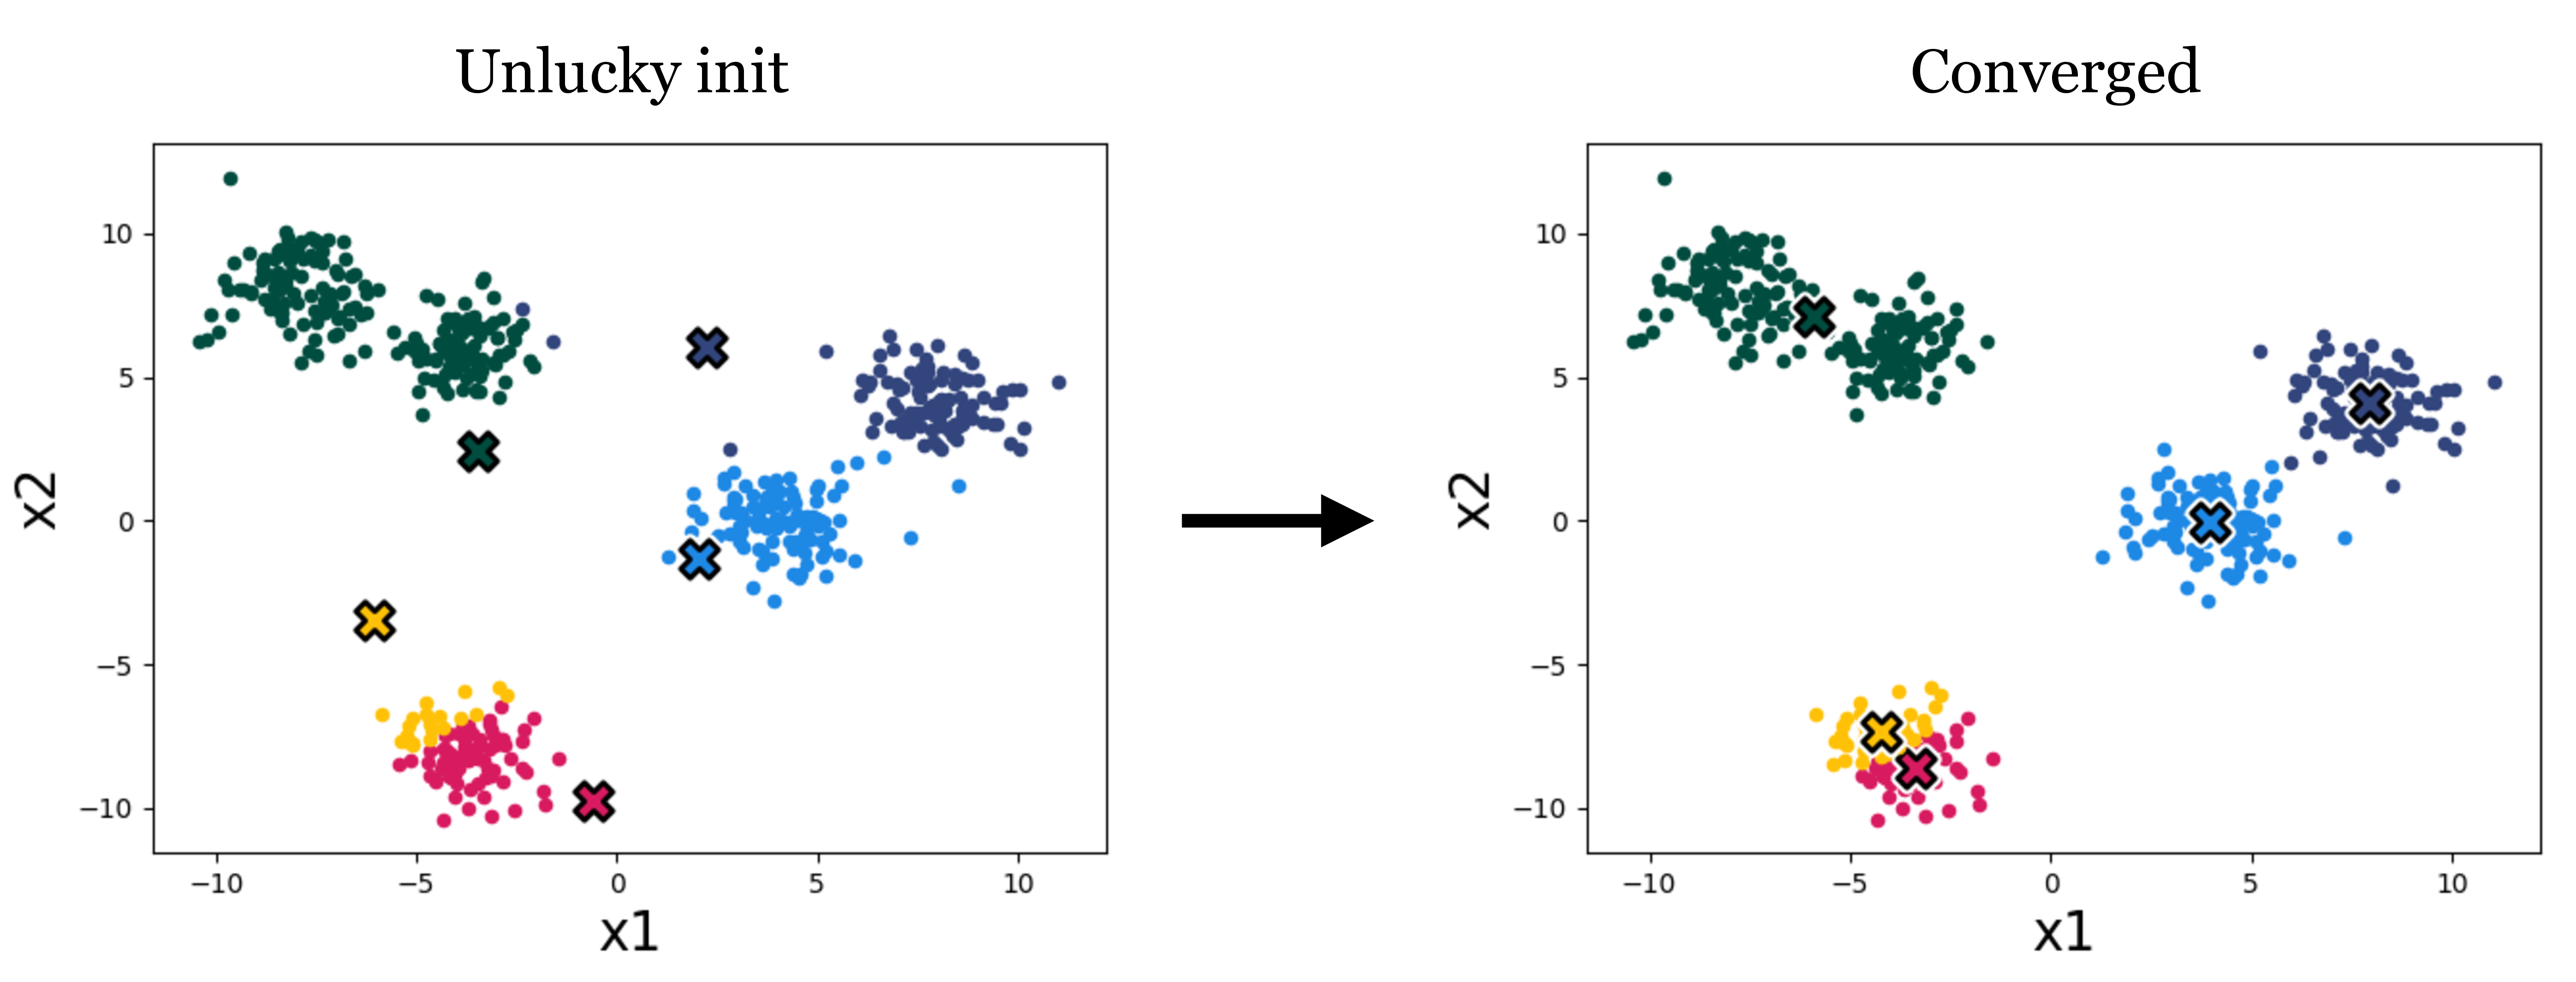
\includegraphics[width=0.8\textwidth]{./figures/kmeans_init.png}
  \caption{With the initialization of the means to the left, the
    yellow and red means end up splitting what perhaps should be one
    cluster in half.}
  \label{fig:kmeans_init}
\end{figure}

A variety of methods have been developed to pick good initializations
(see, for example, the \textit{k-means++} algorithm). One simple
option is to run the standard k-means algorithm multiple times, with
different random initial conditions, and then pick from these the
clustering that achieves the lowest k-means loss.

\subsection{Importance of k}\label{sec-importance_of_k}

A very important parameter in cluster algorithms is the number of
clusters we are looking for. Some advanced algorithms can
automatically infer a suitable number of clusters, but most of the
time, like with k-means, we will have to pick $k$ -- it's a
hyperparameter of the algorithm.

\begin{figure}[h]
  \centering
  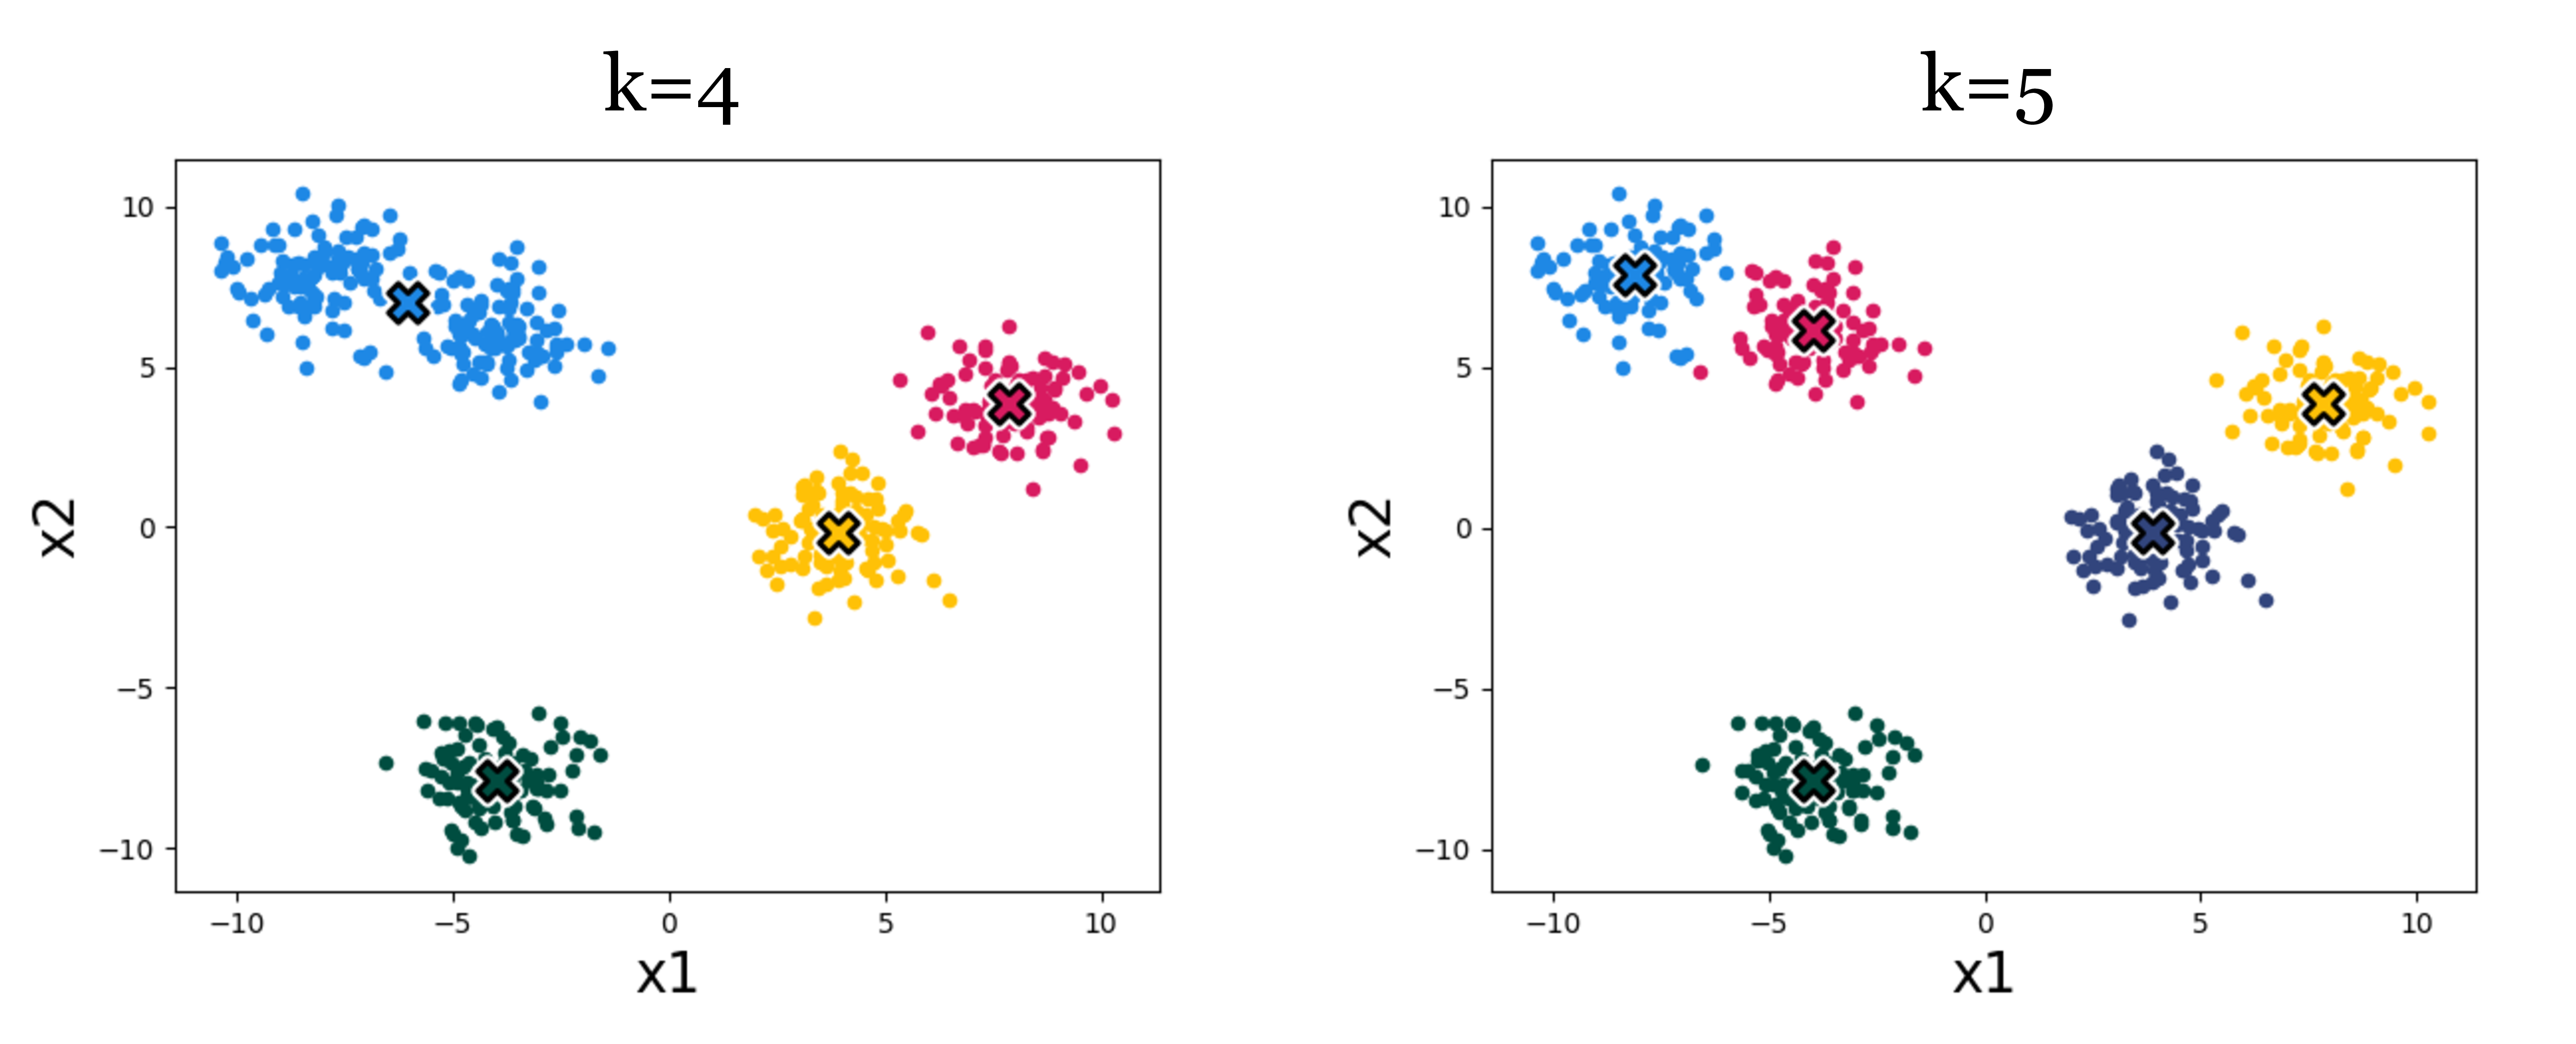
\includegraphics[width=0.67\textwidth]{figures/effect_of_k.png}
  \caption{Example of k-means run on our toy data, with two
    different values of k. Setting k=4, on the left, results in one
    cluster being merged, compared to setting k=5, on the
    right. Which clustering do you think is better? How could you
    decide?}
  \label{fig:effect_of_k}
\end{figure}

Figure~\ref{fig:effect_of_k} shows an example of the effect.  Which
result looks more correct? It can be hard to say! Using higher k we
get more clusters, and with more clusters we can achieve lower
within-cluster variance -- the k-means objective will never increase,
and will typically strictly decrease as we increase k. Eventually, we
can increase k to equal the total number of datapoints, so that each
datapoint is assigned to its own cluster. Then the k-means objective
is zero, but the clustering reveals nothing.  Clearly, then, we cannot
use the k-means objective itself to choose the best value for k. In
Section~\ref{sec-eval}, we will discuss some ways of evaluating the
success of clustering beyond its ability to minimize the k-means
objective, and it's with these sorts of methods that we might decide
on a proper value of k.

Alternatively, you may be wondering: why bother picking a single k?
Wouldn't it be nice to reveal a \textit{hierarchy} of clusterings of
our data, showing both coarse and fine groupings? Indeed
\textit{hierarchical clustering} \index{hierarchical clustering} is another important class of
clustering algorithms, beyond k-means. These methods can be useful for
discovering tree-like structure in data, and they work a bit like this: initially a coarse
split/clustering of the data is applied at the root of the tree, and then as we
descend the tree we split and cluster the data in ever more fine-grained ways. A
prototypical example of hierarchical clustering is to discover a
taxonomy of life, where creatures may be grouped at multiple
granularities, from species to families to kingdoms. You may find a suite of 
clustering algorithms in SKLEARN's 
\href{https://scikit-learn.org/1.5/modules/clustering.html}{cluster} module.


% the
% decision trees we will see later in Chapter~\ref{chap-nonparametric},
% point out: there may be no right answer
%   -- hierarchical call out (different granularities)

% btw there exists a class that finds the whole hierarchy...
% hint at the breadth but focus on k-means

% forge connections to previous topics 
%   -- decision trees and nearest-neighbors
%   -- feature space, autoencoder

\subsection{k-means in feature space}

Clustering algorithms group data based on a notion of
\textit{similarity}, and thus we need to define a \textit{distance metric}
between datapoints. This notion
will also be useful in other machine learning approaches,
such as nearest-neighbor methods that we see in Chapter~\ref{chap-nonparametric}.
In k-means and other methods, our choice of distance
metric can have a big impact on the results we will find.

Our k-means algorithm uses the Euclidean distance, i.e., $\left\Vert
  x^{(i)} - \mu^{(j)} \right\Vert$, with a loss function that is the
square of this distance. We can modify k-means to use different
distance metrics, but a more common trick is to stick with Euclidean
distance but measured in a \textit{feature space}. Just like we did
for regression and classification problems, we can define a feature
map from the data to a nicer feature representation, $\phi(x)$, and
then apply k-means to cluster the data in the\anchorednote{feature
  space.}{In fact, using a simple distance metric in feature space can
  be equivalent to using a more sophisticated distance metric in the
  data space, and this trick forms the basis of \textit{kernel
    methods}, which you can learn about in more advanced machine
  learning classes.}\index{k-means!in feature space}

As a simple example, suppose we have two-dimensional data that is very
stretched out in the first dimension and has less dynamic range in the
second dimension. Then we may want to scale the dimensions so that
each has similar dynamic range, prior to clustering. We could use
standardization, like we did in Chapter~\ref{chap-features}.

If we want to cluster more complex data, like images, music, chemical
compounds, etc., then we will usually need more sophisticated feature
representations. One common practice these days is to use feature
representations learned with a neural network. For example, we can use
an autoencoder to compress images into feature vectors, then cluster
those feature vectors.

%it's best to use a nice feature representation of the data rather
%than the raw format stored on your computer

%As an example, we could use an autoencoder to get the features, as shown here:
% \begin{figure}[h]
%     \centering
%     \includegraphics[width=0.33\textwidth]{example-image-a}
%     \caption{Example of k-means run on some data, in different feature spaces, raw data vs. autoencoder features.}
%     \label{fig:my_label}
% \end{figure}
% connects to week 11's hw too

\section{How to evaluate clustering algorithms}
\label{sec-eval}

\index{clustering!evaluation}
One of the hardest aspects of clustering is knowing how to evaluate
it. This is actually a big issue for all unsupervised learning
methods, since we are just looking for patterns in the data, rather
than explicitly trying to predict target values (which was the case
with supervised learning).

Remember, evaluation metrics are \textit{not} the same as loss
functions, so we can't just measure success by looking at the k-means
loss. In prediction problems, it is critical that the evaluation is on
a held-out test set, while the loss is computed over training data. If
we evaluate on training data we cannot detect overfitting. Something
similar is going on with the example in
Section~\ref{sec-importance_of_k}, where setting k to be too large can
precisely ``fit'' the data (minimize the loss), but yields no general
insight.

One way to evaluate our clusters is to look at the
\textbf{consistency} with which they are found when we run on
different subsamples of our training data, or with different
hyperparameters of our clustering algorithm (e.g.,
initializations). For example, if running on several bootstrapped
samples (random subsets of our data) results in very different
clusters, it should call into question the validity of any of the
individual results.

If we have some notion of what \textbf{ground truth} clusters should
be, e.g., a few data points that we know should be in the same
cluster, then we can measure whether or not our discovered clusters
group these examples correctly.

Clustering is often used for \textbf{visualization} and
\textbf{interpretability}, to make it easier for humans to understand
the data. Here, human judgment may guide the choice of clustering
algorithm. More quantitatively, discovered clusters may be used as input to
\textbf{downstream tasks}. For example, as we saw in the lab, we may fit a different
regression function on the data within each
cluster. Figure~\ref{fig:simpsons_color} gives
an example where this might be useful. In cases like this, the success
of a clustering algorithm can be indirectly measured based on the
success of the downstream application (e.g., does it make the
downstream predictions more accurate).

\begin{figure}[h]
  \centering
  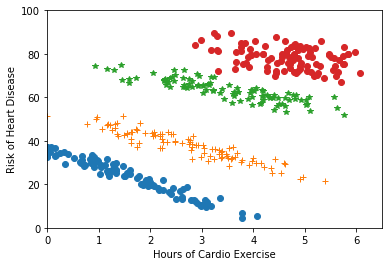
\includegraphics[width=0.35\textwidth]{figures/simpsons_color.png}
  \caption{Averaged across the whole population, risk of heart
    disease positively correlates with hours of exercise. However,
    if we cluster the data, we can observe that there are four
    subgroups of the population which correspond to different age
    groups, and within each subgroup the correlation is negative. We
    can make better predictions, and better capture the presumed
    true effect, if we cluster this data and then model the trend in
    each cluster separately.}
  \label{fig:simpsons_color}
\end{figure}

% Fun stuff to end on?
% High level about unsupervised learning?

% \section{Applications of clustering}

% Clustering has many applications, from visualizing and understanding
% data to efficiently transmitting data over the Internet. Here are a
% few you are now equipped to learn about:

% \begin{itemize}
%     \item ``Vector quantization'' and compression: if we have high-dimensional feature vectors we can summarize them with more compact codewords, i.e., cluster assignments. 
%     \item 
% \end{itemize}

% applications
%  vector quantization; compression

%%% Local Variables:
%%% mode: latex
%%% TeX-master: "top"
%%% End:
